% Theorie: Physikalische Grundlagen von Versuch/Messverfahren, Gleichungen ohne Herleitung knapp erklären
\section[Theorie]{Theorie \textnormal{\cite{doppler}}}
\label{sec:theorie}

Das menschliche Gehör ist für Frequenzen von $\qty{16}{\hertz}$ bis $\qty{20}{\kilo\hertz}$ empfindlich. Außerhalb der unteren Hörschwelle
handelt es sich um Infraschall, der Bereich von $\qty{20}{\kilo\hertz}$ bis $\qty{1}{\giga\hertz}$ wird als Ultraschall bezeichnet. Oberhalb
davon liegen noch die Hyperschallfrequenzen.

\subsection{Doppler-Effekt}

Mit dem Doppler-Effekt wird die Frequenzänderung $\increment \nu$ beschrieben, welche als Resultat der Bewegung von Beobachter
und Quelle mit relativer Geschwindigkeit $v$ zueinander auftritt. Die Wellen mit Ausgangsfrequenz $\nu_0$ breiten sich mit
Schallgeschwindigkeit $c$ im Raum aus. Sollte sich die Quelle in Richtung des Beobachters bewegen, so wächst $\nu$ auf
\begin{equation*}
	\nu_\text{\hspace{-0.2ex}gr} = \pfrac{\nu_0}{1 - \dfrac{\raisebox{-0.8ex}{$v$}}{\raisebox{0.8ex}{$c$}}}
\end{equation*}
an. Entfernt sie sich vom Beobachter, sinkt die Frequenz bis
\begin{equation*}
	\nu_\text{kl} = \pfrac{\nu_0}{1 + \dfrac{\raisebox{-0.8ex}{$v$}}{\raisebox{0.8ex}{$c$}}}
\end{equation*}
ab. Für eine ruhende Quelle erhöht sich $\nu$ nach
\begin{equation*}
	\nu_\text{h} = \nu_0 \left( 1 + \dfrac{\raisebox{-0.8ex}{$v$}}{\raisebox{0.8ex}{$c$}} \right)
\end{equation*}
wenn sich der Beobachter auf die Quelle zubewegt. Vergrößert sich sein Abstand gibt
\begin{equation*}
	\nu_\text{n} = \nu_0 \left( 1 - \dfrac{\raisebox{-0.8ex}{$v$}}{\raisebox{0.8ex}{$c$}} \right)
\end{equation*}
die Verschiebung der Frequenz in niedrigere Bereiche an.

\subsection{Messverfahren}

In der Ultraschalltechnik wird der Doppler-Effekt ausgenutzt, um die Geschwindigkeit von Strömungen zu ermitteln. Medizinisch
finden solche Verfahren zur Bestimmung der Flussgeschwindigkeit in Blutbahnen Anwendung. Wird die Ultraschallwelle mit $\nu_0$ von einem
bewegten Objekt reflektiert, erfährt deren Frequenz gemäß
\begin{equation*}
	\increment \nu = \nu_0 \dfrac{\raisebox{-0.8ex}{$v$}}{\raisebox{0.8ex}{$c$}} \left( \cos \alpha + \cos \beta \right)
\end{equation*}
eine Verschiebung, wobei $\alpha$ und $\beta$ die Winkel von Geschwindigkeit $v$ mit den Normalen von einlaufender und auslaufender
Welle bezeichnen. 

\subsubsection{Impuls-Echo-Ultraschalltechnik}

Für das Impuls-Echo Verfahren sind Sender und Empfänger wie in Abbildung \ref{fig:doppler} angeordnet, sodass immer $\alpha = \beta$ gilt.

\begin{figure}[H]
	\centering
	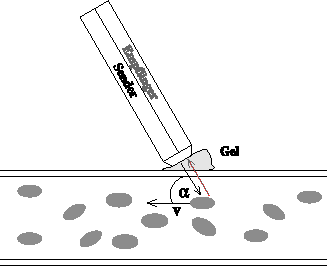
\includegraphics[width=0.6\linewidth]{content/grafik/doppler.pdf}
	\captionsetup{width=\linewidth}
	\caption{Schematische Darstellung der Messanordnung zum Impuls-Echo Verfahren. \cite{doppler}}
	\label{fig:doppler}
\end{figure}

Aus dem vorherigen Zusammenhang ergibt sich in diesem Fall
\begin{equation}
	\increment \nu = 2\nu_0 \dfrac{\raisebox{-0.8ex}{$v$}}{\raisebox{0.8ex}{$c$}} \cos \alpha
	\label{eqn:frequenz}
\end{equation}
als Ausdruck für die Frequenzverschiebung. 

\subsubsection{Piezoelektrische Erzeugung und Detektion}

Wird ein elektrisches Wechselfeld parallel zu einer polaren Achse eines piezoelektrischen Kristalls geschaltet, kann dieser zu Schwingungen im
Ultraschallbereich angeregt werden. Abstimmung von Anregungs- und Eigenfrequenz erlaubt durch Resonanz das Erzeugen großer Wellenamplituden.
Verwenden dieses mit dem Begriff reziproker piezoelektrischer Effekt bezeichneten Phänomens ermöglicht die Nutzung extrem hoher
Schallenergiedichten. Über den umgekehrten Effekt dient der Piezokristall auch als Detektor, indem er durch eintreffende Schallwellen
in Schwingung versetzt wird. Wegen ihrer gleichbleibenden physikalischen Eigenschaften werden solche Messapparturen typischerweise
mithilfe von Quarzen realisiert.

\subsubsection{Doppler-Winkel und akustisches Prisma}

Um präzise Ankopplungswinkel der Ultraschallsonde an die Strömungsrohe zu garantieren, werden Doppler-Prismen mit drei speziell angeordneten
Einstellflächen eingesetzt. 

\begin{figure}[H]
	\centering
	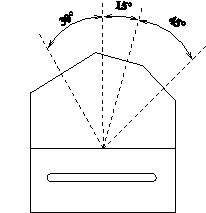
\includegraphics[width=0.4\linewidth]{content/grafik/prisma.pdf}
	\caption{Schema zum an ein Strömungsrohr angesetzten Doppler-Prisma. \cite{doppler}}
	\label{fig:prisma}
\end{figure}

Aus Abbildung \ref{fig:prisma} geht hervor, dass sowohl Abstand und Winkel zur strömenden Flüssigkeit mithilfe des Aufbaus reproduzierbar
definiert sind. Mit den angegebenen Winkeln $\theta$ ergibt sich unter Ausnutzung des Brechungsgesetzes über
\begin{equation}
	\alpha = \qty{90}{\degree} - \arcsin \left( \dfrac{\raisebox{-0.4ex}{$c_\text{L}$}}{\raisebox{0.4ex}{$c_\text{P}$}} \, \sin \theta \right)
	\label{eqn:prisma}
\end{equation}
der Doppler-Winkel, wobei $c_\text{L}$ und $c_\text{P}$ den Schallgeschwindigkeiten von Flüssigkeit und Prismenmaterial entsprechen.
